\documentclass[11pt]{article}
\usepackage[utf8]{inputenc}
\usepackage{amssymb, amsmath, amsthm, changepage, graphicx, caption, subcaption}

\graphicspath{{./images/}}

\title{MAT157 Problem Set 12}
\author{Nicolas}

\newcommand{\R}{\mathbb{R}}

\newcommand{\N}{\mathbb{N}}

\newcommand{\Z}{\mathbb{Z}}

\newcommand{\F}{\mathbb{F}}

\newcommand{\C}{\mathbb{C}}

\newcommand{\Q}{\mathbb{Q}}

\newcommand{\norm}[1]{\left\lVert#1\right\rVert}

\newcommand{\inn}[2]{\langle#1,#2\rangle}

\newenvironment{myproof}
{\begin{proof} \begin{adjustwidth}{3em}{0pt}$ $\par\nobreak\ignorespaces}
{\end{adjustwidth} \end{proof}} 

\begin{document}

\maketitle
\begin{flushleft}

1. a)

\begin{myproof}
Clearly this integral converges if $\lambda \geq 0$ because on $\forall x \in [0,1]$, $(1-x) \geq 0$. Thus $(1-x)^\lambda$ is a well defined, continuous function. However, if $\lambda < 0$ then the integral does not converge. Assume for the sake of contradiction that $\int_0^1 (1-x)^\lambda \,dx$ exists. Then, $\int_{-1}^0(-x)^\lambda \,dx = \int_{-1}^0\frac{1}{(-x)^{|\lambda|}} \,dx$ exists by symmetry. However, this implies that this integral converges, aha! a contradiction. a lil sneaky you...
\end{myproof}

b)

\begin{myproof}
For this integral, $\lambda < 0$ diverges for similar reasons to the other integral. If $\lambda \in \N$ then this function is clearly converges because $\int_{-1}^0(-x^2)^n \,dx$ converges. However, if $\lambda = \frac{p}{2n}, \ p,n \in \N$ with $2n$ as small as possible. If we assume that the integral converges, we must also assume that $\int_{-1}^0(-x^2)^{\frac{p}{2n}} \,dx$ converges. However, we know that $\forall x \in [-1,0)$, $(-x^2) < 0$. Thus $(-x^2)^{\frac{p}{2n}}$ doesn't exist. Because the function does not exist on that interval, the function cannot be convergent. Otherwise (odd rational denominator), this integral converges.
\end{myproof}

\newpage

2. a)

\begin{myproof}
Let $x \in [0, \infty)$.
\begin{align*}
& \ \frac{1+x^2}{\sqrt{1+x^5}} \\
 = & \ \frac{1}{\sqrt{1+x^5}} + \frac{x^2}{\sqrt{1+x^5}} \\
 \leq & \ 1 + \frac{x^2}{\sqrt{1+x^5}} \\
 \leq & \ 1 + \frac{x^2}{\sqrt{x^5}} \\
 = & 1 + \frac{x^2}{x^\frac{2}{5}} \\
 \leq & \ 2
\end{align*}
Therefore, $\forall x \in [0, \infty)$, $\frac{2}{1+x^2} > \frac{1}{\sqrt{1+x^5}}$. Thus if $f:[0, \infty) \to \R$ is RHS and $g:[0, \infty) \to \R$ (the function we want to integrate) is LHS, then $f > g > 0$. Because $f$ is converges, $g$ must also converge.
\end{myproof}

b)

\begin{myproof}
Since $1+ x^2 \cos x$ is a surjection, then consider the first positive value of $x$ such that $1 + x^2 \cos x =0$ and call it $M$. Now consider the function $f:(1,M) \to \R, \ x \mapsto \log(M-x)$. We claim that $\forall x \in (1,M), \ \frac{x}{1+ x^2 \cos x} > \log (M-x)$. However, if $\exists x \in (0,M)$ such that $\frac{x}{1+ x^2 \cos x} < \log (M-x)$ this contradicts the fact that $\log$ is \textbf{SLOW}.  Thus, because $\int_1^M \log(M-x) \,dx = \infty$, $\int_1^M \frac{x}{1+x^2 \cos x \,dx} = \infty$, meaning that $\int_0^\infty \frac{x}{1+x^2 \cos x} \,dx = \infty$ and is therefore, divergent.
\end{myproof}

c)

\begin{myproof}
Consider $f:(1, \infty) \to \R, \ f(x) = \frac{1}{x^2} + 1$. $\forall x \in (1,\infty) f(x) \geq 1 \geq \sin (\frac{1}{x^2}) > 0$. Thus because $\int_1^\infty f(x) \,dx$ converges, that implies that $\int_1^\infty \sin (\frac{1}{x^2}) \,dx$ also converges.
\end{myproof}

\newpage

3. a)

\begin{myproof}
Consider the primative, $F$, of the function $f(x) = \frac{1}{\sin^2 x}$. As you can verify $F(x) = - \frac{1}{\tan x}$. Thus, by \textbf{FTC} $\lim_{x \to 0^+} \int_{Ax}^{Bx} \frac{1}{\sin^2 t} \,dt = \lim_{x \to 0^+} F(x)]_{Ax}^{Bx} = \lim_{x \to 0^+} F(Bx) - F(Ax)$. Thus, we must simply evaluate the $\lim_{x \to 0^+} \frac{1}{\tan (Ax)} - \frac{1}{\tan (Bx)} = \lim_{x \to 0^+} \frac{\tan (Bx) - \tan (Ax)}{\tan (Ax) \tan (Bx)}$ As $x$ arbitrarily small, the numerator is always positive, while the denominator goes to zero and is positive. Thus, $\int_{Ax}^{Bx} \frac{1}{\sin^2 t} \,dt = \infty$.
\end{myproof}

b)

\begin{myproof}
$\lim_{x \to 0^+} x \int_{Ax}^{Bx} f(t) \,dt = \lim_{x \to 0^+} \frac{\int_{Ax}^{Bx} f(t) \,dt}{x^{-1}}$. This is indeterminate form $\frac{\infty}{\infty}$ so we can apply \textit{l'hopital's rule}. $\frac{d}{dx} \int_{Ax}^{Bx} f(t) \,dt = \frac{d}{dx} (\int_{0}^{Bx} f(t) \,dt - \int_{0}^{Ax} f(t) \,dt) = \frac{B}{ \sin^2 (Bx)} - \frac{A}{ \sin^2 (Ax)}$. Thus, $\lim_{x \to 0^+} x \int_{Ax}^{Bx} f(t) \,dt = \frac{ \frac{B}{ \sin^2 (Bx)} - \frac{A}{ \sin^2 (Ax)}}{-(0)^{-2}} = 0$ as desired.
\end{myproof}

\newpage

4. a)

\begin{myproof}
Let $M_i = f(t_i)$ and $m_i=f(t_{i-1})$. Notice that $t_i - t_{i-1} = a + i\frac{b-a}{n} - a - (i-1)\frac{b-a}{n}$. Also notice that $\sum_{i=1}^n M_i - m_i = f(t_1) - f(t_0) + f(t_2) - f(t_1) + \cdots + f(t_n) - f(t_{n-1}) = |f(b)-f(a)|$ because the series telescopes.
\begin{align*}
U(f,P_n) - L(f,P_n) = & \ \sum_{i=1}^n(t_i - t_{i-1})M_i-m_i \\
= & \ \frac{b-a}{n} \sum_{i=1}^n M_i - m_i \\
= & \ \frac{b-a}{n}|f(b) - f(a)|
\end{align*}
As desired.
\end{myproof}

b)

\begin{myproof}
Let $\varepsilon > 0$ let $N > \frac{\varepsilon}{\sup \{M_i - m_i| i \in \{1,...,n\} \} \cdot (b-a)}$. Thus for every $n > N$, $U(f,P_n) - L(f,P_n) = \frac{b-a}{n}\sum_{i=1}^nM_i - m_i < \frac{b-a}{N}\sup \{M_i - m_i| i \in \{1,...,n\} \} < \varepsilon$. Thus, the limits are of upper and lower Riemann sums are equal, thus the whole function is integrable.
\end{myproof}

c)
\begin{myproof}
Consider $\lim_{n \to \infty} n^d \sum_{i=0}^n \frac{1}{(i+n)^{d+1}} = \lim_{x \to \infty} \sum_{i=0}^n \frac{n^d}{(i+n)^{d+1}} $ However, as $x$ goes to infinity, we are left with $\frac{\infty}{\infty}$ which is an indeterminate form. Notice, that the expression is in indeterminate form for any $d \in \N$. Thus we can apply \textit{l'hopital's rule} and differentiate in respect to $n$, $d$ times. Thus $\frac{d}{dn^d} n^d=d!$ and $\frac{d}{dn^d} (a + n)^{d+1} = (d+1)!(a+n), \ a \in \N$. Thus, $\lim_{n \to \infty} \frac{d}{dn^d} \frac{d!}{(d+1)!(a+n)}= \lim_{n \to \infty} \frac{1}{(d+1)(a+n)} =0$. Thus, $\lim_{n \to \infty}  n^d \sum_{i=0}^n \frac{1}{(i+n)^{d+1}} = \lim_{n \to \infty} \sum_{i=1}^n 0 = 0$.
\end{myproof}

\newpage

5.

\begin{myproof}
Consider the function 
\begin{align*}
f: \R \to \R, \ f(x) = \begin{cases} \frac{1}{n^2} (x-10n-\frac{1}{n^2}) & \ \text{ if } 0 < 10n-x < \frac{1}{n^2}, \ \forall n \in \N \\ -\frac{1}{n^2} (x-10n-\frac{1}{n^2}) &  \ \text{ if } 0 > x-10n > -\frac{1}{n^2}, \ \forall n \in \N \\ 0 & \ \text{ otherwise} \end{cases}
\end{align*}
Clearly, we can see that $f$ is non-negative everywhere, and if $0 < 10n-x < \frac{1}{n^2}, \ \forall n \in \N$ then $f$ is locally the same as a degree 1 polynomial, which is continuous, and similarly for $0 > x-10n > -\frac{1}{n^2}$. If $x$ is otherwise, then $f$ is locally the zero function which is continuous. \\
\bigskip
Now consider $\lim_{x \to \infty} \int_0^x f(t) \,dt$. Let $\varepsilon > 0$ choose $N > S$ such that the $S$'th partial sum of $|L-\sum_{n = 1}^{S}\frac{1}{n^2}| < \varepsilon$. We know this converges because $\int_1^\infty \frac{1}{x^2} \,dx$ converges. Thus if $x > N$, we know that $\int_0^x f(t) \,dt = \int_0^{11}f(t) \,dt + \int_{11}^{21}f(t) + \cdots + \int_c^x f(t) \,dt \geq \sum_{n = 1}^{N}\frac{1}{n^2}$. However, we know that there exists $N' > x > N$ such that $\sum_{n = 1}^{N}\frac{1}{n^2} \leq \int_0^x f(t) \,dt < \sum_{n = 1}^{N'}\frac{1}{n^2}$. Since $N' > N$, this implies that $|L - \sum_{n=1}^{N'} \frac{1}{n^2}| < \varepsilon$ which gives us $|L - \int_0^x f(t) \,dt| < \varepsilon$  as desired.\\
\bigskip
$\lim_{x \to \infty}f(x)$ does not exist because if $\varepsilon = \frac{1}{2}$ no matter how we choose $N$ there exists $x > y > N$ such that $f(x) = 1$ and $f(y) = 0$. Thus if $|L-f(x)|< \varepsilon$ that means that $|L-f(y)| \geq \varepsilon$, implying the limit does not exist.\\
\bigskip
This is the graph of my function (\textit{* not to scale}):
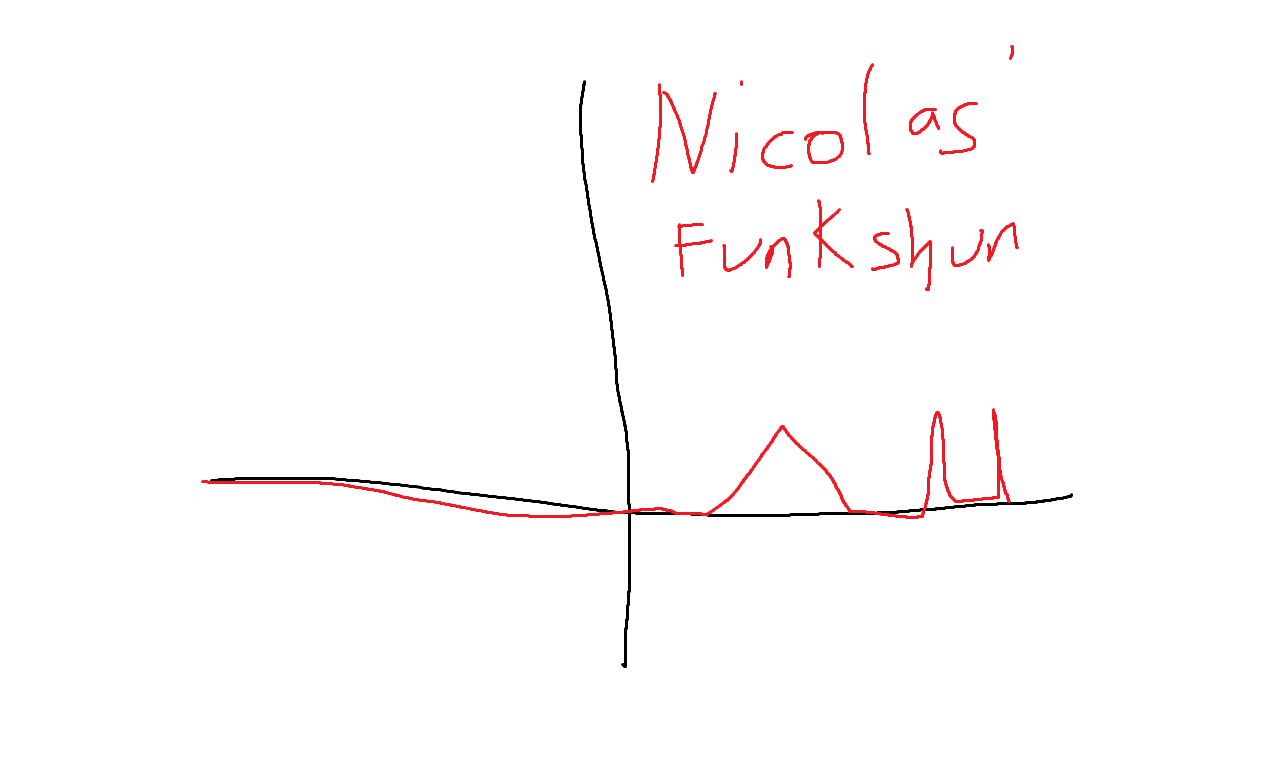
\includegraphics[width=\textwidth]{nicofunkshun.png}
\end{myproof}

\end{flushleft}
\end{document}